

\documentclass[12pt]{article}
\usepackage[margin=1in]{geometry}


%===============================================================================
%================================== PACKAGES ===================================
%===============================================================================

% For using float option H that places figures 
% exatcly where we want them
\usepackage{float}
% makes figure font bold
\usepackage{caption}
\captionsetup[figure]{labelfont=bf}
% For text generation
\usepackage{lipsum}
% For drawing
\usepackage{tikz}
% For smaller or equal sign and not divide sign
\usepackage{amssymb}
% For the diagonal fraction
\usepackage{xfrac}
% For enumerating exercise parts with letters instead of numbers
\usepackage{enumitem}
% For dfrac, which forces the fraction to be in display mode (large) e
% even in math mode (small)
\usepackage{amsmath}
% For degree sign
\usepackage{gensymb}
% For "\mathbb" macro
\usepackage{amsfonts}
% For positioning 
\usepackage{indentfirst}
\usetikzlibrary{shapes,positioning,fit,calc}
% for adjustwidth environment
\usepackage{changepage}
% for arrow on top
\usepackage{esvect}
% for mathbb 1
\usepackage{bbm}
% for mathsrc
\usepackage[mathscr]{eucal}
% For degree sign
\usepackage{gensymb}
% For quotes
\usepackage{csquotes}
% For vertical lines
\usepackage{mathtools}
% For cols
\usepackage{multicol}

% for tikz
\usepackage{pgfplots}
\pgfplotsset{compat=1.18}
\usepackage{amsmath}
\usepgfplotslibrary{groupplots}


%===============================================================================
%==================================== FONTS ====================================
%===============================================================================


% Mathcal
\newcommand{\acal}{\mathcal{A}}
\newcommand{\bcal}{\mathcal{B}}
\newcommand{\ccal}{\mathcal{C}}
\newcommand{\dcal}{\mathcal{D}}
\newcommand{\ecal}{\mathcal{E}}
\newcommand{\fcal}{\mathcal{F}}
\newcommand{\gcal}{\mathcal{G}}
\newcommand{\hcal}{\mathcal{H}}
\newcommand{\ical}{\mathcal{I}}
\newcommand{\jcal}{\mathcal{J}}
\newcommand{\kcal}{\mathcal{K}}
\newcommand{\lcal}{\mathcal{L}}
\newcommand{\mcal}{\mathcal{M}}
\newcommand{\ncal}{\mathcal{N}}
\newcommand{\ocal}{\mathcal{O}}
\newcommand{\pcal}{\mathcal{P}}
\newcommand{\qcal}{\mathcal{Q}}
\newcommand{\rcal}{\mathcal{R}}
\newcommand{\scal}{\mathcal{S}}
\newcommand{\tcal}{\mathcal{T}}
\newcommand{\ucal}{\mathcal{U}}
\newcommand{\vcal}{\mathcal{V}}
\newcommand{\wcal}{\mathcal{W}}
\newcommand{\xcal}{\mathcal{X}}
\newcommand{\ycal}{\mathcal{Y}}
\newcommand{\zcal}{\mathcal{Z}}

% Mathfrak
\newcommand{\afrak}{\mathfrak{A}}
\newcommand{\bfrak}{\mathfrak{B}}
\newcommand{\cfrak}{\mathfrak{C}}
\newcommand{\dfrak}{\mathfrak{D}}
\newcommand{\efrak}{\mathfrak{E}}
\newcommand{\ffrak}{\mathfrak{F}}
\newcommand{\gfrak}{\mathfrak{G}}
\newcommand{\hfrak}{\mathfrak{H}}
\newcommand{\ifrak}{\mathfrak{I}}
\newcommand{\jfrak}{\mathfrak{J}}
\newcommand{\kfrak}{\mathfrak{K}}
\newcommand{\lfrak}{\mathfrak{L}}
\newcommand{\mfrak}{\mathfrak{M}}
\newcommand{\nfrak}{\mathfrak{N}}
\newcommand{\ofrak}{\mathfrak{O}}
\newcommand{\pfrak}{\mathfrak{P}}
\newcommand{\qfrak}{\mathfrak{Q}}
\newcommand{\rfrak}{\mathfrak{R}}
\newcommand{\sfrak}{\mathfrak{S}}
\newcommand{\tfrak}{\mathfrak{T}}
\newcommand{\ufrak}{\mathfrak{U}}
\newcommand{\vfrak}{\mathfrak{V}}
\newcommand{\wfrak}{\mathfrak{W}}
\newcommand{\xfrak}{\mathfrak{X}}
\newcommand{\yfrak}{\mathfrak{Y}}
\newcommand{\zfrak}{\mathfrak{Z}}

% Mathscr
\newcommand{\ascr}{\mathscr{A}}
\newcommand{\bscr}{\mathscr{B}}
\newcommand{\cscr}{\mathscr{C}}
\newcommand{\dscr}{\mathscr{D}}
\newcommand{\escr}{\mathscr{E}}
\newcommand{\fscr}{\mathscr{F}}
\newcommand{\gscr}{\mathscr{G}}
\newcommand{\hscr}{\mathscr{H}}
\newcommand{\iscr}{\mathscr{I}}
\newcommand{\jscr}{\mathscr{J}}
\newcommand{\kscr}{\mathscr{K}}
\newcommand{\lscr}{\mathscr{L}}
\newcommand{\mscr}{\mathscr{M}}
\newcommand{\nscr}{\mathscr{N}}
\newcommand{\oscr}{\mathscr{O}}
\newcommand{\pscr}{\mathscr{P}}
\newcommand{\qscr}{\mathscr{Q}}
\newcommand{\rscr}{\mathscr{R}}
\newcommand{\sscr}{\mathscr{S}}
\newcommand{\tscr}{\mathscr{T}}
\newcommand{\uscr}{\mathscr{U}}
\newcommand{\vscr}{\mathscr{V}}
\newcommand{\wscr}{\mathscr{W}}
\newcommand{\xscr}{\mathscr{X}}
\newcommand{\yscr}{\mathscr{Y}}
\newcommand{\zscr}{\mathscr{Z}}

% Mathbb
\newcommand{\abb}{\mathbb{A}}
\newcommand{\bbb}{\mathbb{B}}
\newcommand{\cbb}{\mathbb{C}}
\newcommand{\dbb}{\mathbb{D}}
\newcommand{\ebb}{\mathbb{E}}
\newcommand{\fbb}{\mathbb{F}}
\newcommand{\gbb}{\mathbb{G}}
\newcommand{\hbb}{\mathbb{H}}
\newcommand{\ibb}{\mathbb{I}}
\newcommand{\jbb}{\mathbb{J}}
\newcommand{\kbb}{\mathbb{K}}
\newcommand{\lbb}{\mathbb{L}}
\newcommand{\mbb}{\mathbb{M}}
\newcommand{\nbb}{\mathbb{N}}
\newcommand{\obb}{\mathbb{O}}
\newcommand{\pbb}{\mathbb{P}}
\newcommand{\qbb}{\mathbb{Q}}
\newcommand{\rbb}{\mathbb{R}}
\newcommand{\sbb}{\mathbb{S}}
\newcommand{\tbb}{\mathbb{T}}
\newcommand{\ubb}{\mathbb{U}}
\newcommand{\vbb}{\mathbb{V}}
\newcommand{\wbb}{\mathbb{W}}
\newcommand{\xbb}{\mathbb{X}}
\newcommand{\ybb}{\mathbb{Y}}
\newcommand{\zbb}{\mathbb{Z}}


%===============================================================================
%=============================== SPECIAL SYMBOLS ===============================
%===============================================================================


% Orbit (group theory)
\newcommand{\orbit}{\mathcal{O}}
% Normal group
\newcommand{\normal}{\mathcal{N}}
% Indicator function
\newcommand{\indicator}{\mathbbm{1}}
% Laplace transform
\newcommand{\laplace}[1]{\mathcal{L}}
% Epsilon shorthand
\newcommand{\eps}{\varepsilon}
% Omega
\newcommand{\om}{\omega}
\newcommand{\Om}{\Omega}

%===============================================================================
%================================== OPERATORS ==================================
%===============================================================================


% Inverse exponent
\newcommand{\inv}[0]{^{-1}}
% Overline bar
\newcommand{\olsi}[1]{\,\overline{\!{#1}}}
% Less than or equal slanted
\newcommand{\seqs}{\leqslant}
% Greater or equal slanted
\newcommand{\geqs}{\geqslant}
% Subset or equal
\newcommand{\sub}{\subseteq}
% Proper subset
\newcommand{\prosub}{\subset}
% from
\newcommand{\from}{\leftarrow}

% Parantheses
\newcommand{\para}[1]{\left( #1 \right)}
% Curly Braces
\newcommand{\curl}[1]{\left\{ #1 \right\}}
% Brackets
\newcommand{\brac}[1]{\left[ #1 \right]}
% Angled Brackets
\newcommand{\ang}[1]{\left\langle #1 \right\rangle}
% Norm
\newcommand{\norm}[1]{\left\| #1 \right\|}

% Piece wise (use \\ between cases)
\newcommand{\piecewise}[1]{\begin{cases} #1 \end{cases}}

% Bold symbol shorthand
\newcommand{\bl}{\boldsymbol}

% Vertical space
\newcommand{\vs}[1]{\vspace{#1 pt}}
% Horizontal ertical space
\newcommand{\hs}[1]{\hspace{#1 pt}}


%===============================================================================
%============================== TEXT BASED SYMBOLS =============================
%===============================================================================


% Radians
\newcommand{\rad}{\text{rad}}
% Least Common Multiple
\newcommand{\lcm}{\text{lcm}}
% Automorphism
\newcommand{\Aut}{\text{Aut}}
% Variance
\newcommand{\var}{\text{Var}}
% Covariance
\newcommand{\cov}{\text{Cov}}
% Cofactor (matrix)
\newcommand{\cof}{\text{Cof}}
% Adjugate (matrix)
\newcommand{\adj}{\text{Adj}}
% Trace (matrix)
\newcommand{\tr}{\text{tr}}
% Standard deviation
\newcommand{\std}{\text{Std}}
% Correlation coefficient
\newcommand{\corr}{\text{Corr}}
% Sign
\newcommand{\sign}{\text{sign}}

% And text
\newcommand{\AND}{\text{ and }}
% Or text 
\newcommand{\OR}{\text{ or }}
% If text
\newcommand{\IF}{\text{ if }}
% When text
\newcommand{\WHEN}{\text{ when }}
% Then text
\newcommand{\THEN}{\text{ then }}

% 1st
\newcommand{\st}[1]{#1^{\text{st}}}
% 2nd
\newcommand{\nd}[1]{#1^{\text{nd}}}
% 3rd
\newcommand{\rd}[1]{#1^{\text{rd}}}
% nth
\newcommand{\nth}[1]{#1^{\text{th}}}


%===============================================================================
%========================= PROBABILITY AND STATISTICS ==========================
%===============================================================================


% Permutation
\newcommand{\perm}[2]{{}^{#1}\!P_{#2}}
% Combination
\newcommand{\comb}[2]{{}^{#1}C_{#2}}

% Baye's risk
\newcommand{\risk}[1]{\mathscr{R}_{#1}}
% Baye's optimal risk
\newcommand{\riskOptimal}[1]{\mathscr{R}_{#1}^*}
% Baye's empirical risk
\newcommand{\riskEmpirical}[2]{\hat{\mathscr{R}}_{#1}^{#2}}


%===============================================================================
%=================================== CALCULUS ==================================
%===============================================================================


% d over d derivative
\newcommand{\dd}[2]{\dfrac{d#1}{d#2}}
% partial d over d derivative
\newcommand{\partialdd}[2]{\dfrac{\partial #1}{\partial #2}}
% delta d over d derivative
\newcommand{\deltadd}[2]{\dfrac{\Delta #1}{\Delta #2}}

% Integration between a and b
\newcommand{\integral}[4]{\int_{#1}^{#2} #3 \, #4}
% Integration in some space 
\newcommand{\boundIntegral}[2]{\int_{#1} #2 \, d#1}

% Limit
\newcommand{\limit}[3]{\lim_{#1 \to #2} #3}


%===============================================================================
%================================  BIG SYMBOLS  ================================
%===============================================================================


% Sum
\newcommand{\sumof}[2]{\sum_{#1}^{#2}}
% Product
\newcommand{\productof}[2]{\prod_{#1}^{#2}}
% Union
\newcommand{\unionof}[2]{\bigcup_{#1}^{#2}}
% Intersection
\newcommand{\intersectionof}[2]{\bigcap_{#1}^{#2}}
% Or
\newcommand{\orof}[2]{\bigvee_{#1}^{#2}}
% And
\newcommand{\andof}[2]{\bigwedge_{#1}^{#2}}


%===============================================================================
%=============================== LINEAR ALGEBRA ================================
%===============================================================================


% Bold vector arrow
\newcommand{\bv}[1]{\vec{\mathbf{#1}}}

% Matrix or vector (use // for column, & for row) 
% with brackets
\newcommand{\bmat}[1]{\begin{bmatrix} #1 \end{bmatrix}}
% Matrix or vector (use // for column, & for row) 
% with curved brackets
\newcommand{\pmat}[1]{\begin{pmatrix} #1 \end{pmatrix}}
% Matrix or vector (use // for column, & for row) 
% with lines on either side 
\newcommand{\lmat}[1]{\begin{vmatrix} #1 \end{vmatrix}}
% Matrix or vector (use // for column, & for row) 
% with curly braces
\newcommand{\cmat}[1]{\begin{Bmatrix} #1 \end{Bmatrix}}
% Matrix or vector (use // for column, & for row) 
% with no braces
\newcommand{\mat}[1]{\begin{matrix} #1 \end{matrix}}


%===============================================================================
%================================ LARGE OBJECTS ================================
%===============================================================================

% Multiple lines
\newcommand{\multiline}[1]{
\begin{align*}
    #1
\end{align*}
}

% Multiple lines with equation numbers
\newcommand{\eqmultiline}[1]{
\begin{align*}
    #1
\end{align*}
}

% Color
\newcommand{\colorText}[2]{
\begingroup
\color{#1}
    #2
\endgroup
}

% Centered figure
\newcommand{\centerFigure}[2]{
    \begin{figure}[h]
        \centering
            #1
        \caption{#2}
    \end{figure}
}

% Tikz figure
\newcommand{\tikzGraphic}[1]{
    \begin{center}
    \begin{tikzpicture}
        #1
    \end{tikzpicture}
    \end{center}
}

% Enumerate numbers (seperate by \item)
\newcommand{\numbers}{\textbf{\number*)}}

% Enumerate letters (seperate by \item)
\newcommand{\letters}{\textbf{\alph*)}}

\title{%
    \Huge Abstract Algebra \\
    \large by \\
    \Large Dummit and Foote \\~\\
    \huge Part 0: Preliminaries \\
    \LARGE Chapter 0: Preliminaries \\
    \Large Section 1: Basics
}
\date{2024-03-17}
\author{Michael Saba}

\begin{document}
    \pagenumbering{gobble}
    \maketitle
    \newpage    
    \setlength{\parindent}{0pt}
    \pagenumbering{arabic}

    This section just introduces some concepts in set theory. \\

    \subsection*{Sets}

    A \textbf{set} is an unordered collection of elements,
    where we don't care about repetition.
    So these sets are all equivalent
    \[ \{1, 2, 3\} = \{ 1, 3, 2\} = \{ 1, 1, 2, 3, 3 \}  \]
    We usually use capital letters such as $A$ to denote sets. \\
    When $a$ is an element in a set $A$,
    we say $a \in A$, and if $a$ isn't an element of $A$,
    we say $a \notin A$. \\
    We don't necessarily need to list all elements of a set
    to define it, we can instead define it like this
    \[ B = \{ a \in A \mid \dots \text{ condition on $a$ } \dots \} \]
    Examples of a set includes the set of integers $\Z$,
    the set of natural numbers $\N$,
    the set of rational numbers $\Q$,
    and the set of real numbers $\R$. \\

    There is a unique set that contains no elements,
    and it is called the \textbf{empty set},
    and represented by the symbol $\emptyset$. \\
    
    The \textbf{cardinality} of a set $A$ is the number of (unique)
    elements in it.
    We denote the cardinality of $A$ as $|A|$. \\

    The \textbf{union} of two sets is the set of elements
    that feature in either sets.
    A union between $A$ and $B$ is denoted as $A \cup B$, such that
    \[ A \cup B = \{ a \mid a \in A \text{ or } a \in B \} \]
    On the other hand, an \textbf{intersection} of two sets is the set of
    elements that feature in both sets.
    An intersection between $A$ and $B$ is denoted as $A \cap B$, such that
    \[ A \cap B = \{ a \mid a \in A \text{ and } a \in B \} \]
    Finally, the \textbf{difference} between two sets $A$ and $B$
    is the set of elements in $A$ not in $B$.
    The difference between $A$ and $B$ is denoted as $A - B$,
    (sometimes $A \setminus B$), such that
    \[ A - B = \{ a \mid a \in A \text{ and } a \notin B \} \]
    \\

    A set $B$ is \textbf{subset} of a set $A$
    if all elements of $B$ are in $A$.
    We say $B \subseteq A$.
    Note that for any set $A$, $A \subseteq A$. \\
    Furthermore, the set $B$ is said to be a
    \textbf{proper subset} of $A$ if $B \subseteq A$
    and $|B| < |A|$.
    In other words, a proper subset is one that is
    contained in another set, but isn't the set itself.
    We denote a proper subset using $B \subset A$.
    If $B$ isn't a proper subset of $A$,
    but is a subset of $A$, then $A = B$. \\

    One way to prove that two sets $A$ and $B$
    are equal is to show that $A \subseteq B$
    and that $B \subseteq A$;
    if both sets are contained in each other,
    then they have to be the same set,
    for the same reason that if $x \leqslant y$
    and $y \leqslant x$, then $x = y$. \\ 
    Another way of thinking about this is this. 
    We know that $A = B$
    means that $a \in A$ if and only if $a \in B$.
    This implies that if $a \in A$ then $a \in B$,
    and that if $a \in B$ then $a \in A$.
    The first statement basically means that $A \subseteq B$,
    and the second means that $B \subseteq A$. \\

    The \textbf{cartesian product} of two non-empty sets $A$ and $B$
    is the set $A \times B$ defined as
    \[ A \times B = \{ (a, b) \mid
    \forall a \in A \text{ and } \forall b \in B \} \]
    Here, $(a, b)$ is an \textbf{ordered pair};
    similar to a set, but the order matters,
    and we care about repetition. \\
    Moreover, $A \times B \times C$
    is the set of tuples $(a, b, c)$
    for all elements $a \in A$, $b \in B$, and $c \in C$. \\
    This can be extended for any number of non-empty sets.
    Note however that
    \[ A \times B \times C \quad \neq \quad (A \times B) \times C 
    \quad \neq \quad A \times (B \times C) \]
    as the the second set is the set of
    ordered pairs $((a, b),  c)$,
    and third set is the set of
    the ordered pairs $(a, (b, c))$,
    neither of which is equivalent,
    and neither of which is a $3$-tuple $(a, b, c)$. \\


    \subsection*{Functions}

    A \textbf{relation} between non-empty sets
    $A$, $B$, $C \dots$ is a subset
    of their cartesian product $A \times B \times C \dots$.
    In other words, it's a set of associations between elements
    of the sets.
    Each element of a relation is thus the tuple $(a, b, c \dots)$. \\
    A \textbf{binary relation}
    is specifically a relation between two non-empty sets $A$ and $B$.
    An element of a relation $(a, b)$ where $a \in A$ and $b \in b$
    can also be written as $a \sim b$. \\

    A \textbf{function} is a specific type of relation, 
    where all of the elements from set $A$
    are each associated with exatcly one element from set $B$.
    So $\forall a \in A$,
    a function $f$ from $A$ to $B$
    must contain a single ordered pair $(a, b)$ for some $b \in B$.
    Note that not every $b \in B$ has to be an image in the function.
    We denote such a function $f: A \rightarrow B$.
    We can also use $A \stackrel{f}{\rightarrow} B$. \\
    For specific element mappings,
    we use $f(a) = b$, or $f: a \mapsto b$. \\
    Also note that if a relation  $f: A \rightarrow B$
    satisfies these properties,
    we say it is \textbf{well defined},
    meaning it is a real function.
    So two ways in which a relation could fail to be well defined
    is if an element of $A$ does not have an image in $f$,
    or is it has more than one image in $f$.
    One way to express that is to say that
    if $a = b$, then $f(a) = f(b)$.

    \begin{figure}[H]
        \centering

        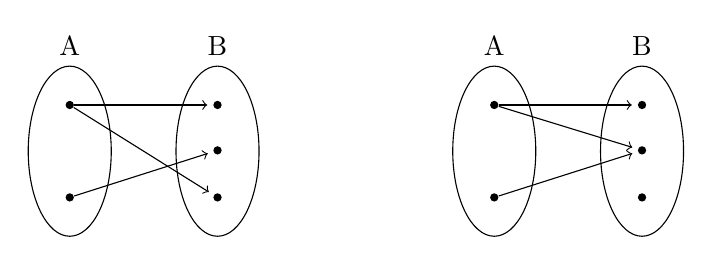
\begin{tikzpicture}
            [
            group/.style={ellipse, draw, minimum height=50pt,
                minimum width=30pt, label=above:#1},
            my dot/.style={circle, fill, minimum width=3pt, inner sep=0pt}
            ]
            \node (a) [my dot=a] {};
            \node (b) [below= 30pt of a, my dot=b] {};
            \node (c) [right=50pt of a, my dot=c] {};
            \node (d) [below= 13pt of c, my dot=d] {};
            \node (e) [right= 50pt of b, my dot=e] {};

            % Replicated nodes
            \node (a2) [right=150pt of a, my dot=a] {};
            \node (b2) [below=30pt of a2, my dot=b] {};
            \node (c2) [right=50pt of a2, my dot=c] {};
            \node (d2) [below=13pt of c2, my dot=d] {};
            \node (e2) [right=50pt of b2, my dot=e] {};

            \foreach \i/\j in {a/c,a/e,b/d}
            \draw [->, shorten >=2pt] (\i) -- (\j);
            \node [fit=(a) (b), group=A] {};
            \node [fit=(d) (c) (e), group=B] {};

            \foreach \i/\j in {a2/c2,a2/d2,b2/d2}
            \draw [->, shorten >=2pt] (\i) -- (\j);
            \node [fit=(a2) (b2), group=A] {};
            \node [fit=(d2) (c2) (e2), group=B] {};
        \end{tikzpicture}  

        \caption{\label{fig:figure1} Examples of functions.}
    \end{figure}

    \begin{figure}[H]
        \centering

        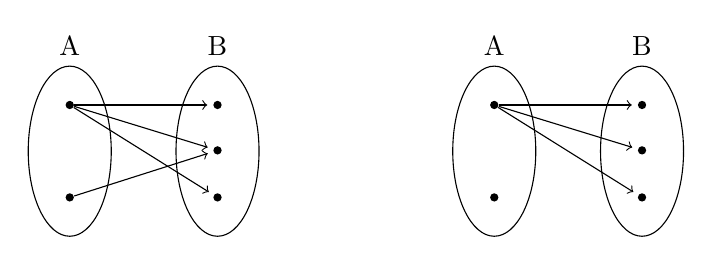
\begin{tikzpicture}
            [
            group/.style={ellipse, draw, minimum height=50pt, 
                minimum width=30pt, label=above:#1},
            my dot/.style={circle, fill, minimum width=3pt, inner sep=0pt}
            ]
            \node (a) [my dot=a] {};
            \node (b) [below= 30pt of a, my dot=b] {};
            \node (c) [right=50pt of a, my dot=c] {};
            \node (d) [below= 13pt of c, my dot=d] {};
            \node (e) [right= 50pt of b, my dot=e] {};

            % Replicated nodes
            \node (a2) [right=150pt of a, my dot=a] {};
            \node (b2) [below=30pt of a2, my dot=b] {};
            \node (c2) [right=50pt of a2, my dot=c] {};
            \node (d2) [below=13pt of c2, my dot=d] {};
            \node (e2) [right=50pt of b2, my dot=e] {};

            \foreach \i/\j in {a/c,a/e,b/d,a/d}
            \draw [->, shorten >=2pt] (\i) -- (\j);
            \node [fit=(a) (b), group=A] {};
            \node [fit=(d) (c) (e), group=B] {};

            \foreach \i/\j in {a2/c2,a2/d2,a2/e2}
            \draw [->, shorten >=2pt] (\i) -- (\j);
            \node [fit=(a2) (b2), group=A] {};
            \node [fit=(d2) (c2) (e2), group=B] {};
        \end{tikzpicture}  

        \caption{
            \label{fig:figure1} Examples of relations 
            that aren't functions.
        }
    \end{figure}
  
    When we have $f: A \rightarrow B$
    or $A \stackrel{f}{\rightarrow} B$,
    we call $A$ the \textbf{domain} of $f$
    and $B$ the \textbf{codomain}. \\
    Note that $f$ being well defined means each element of $A$
    has exactly one mapping in $B$, not that each element of $B$
    is associated with an element in $A$.
    However, the set of all elements in $B$ that do have
    such an association
    is the \textbf{image} of $A$ under $f$,
    sometimes also the \textbf{range} of $f$.
    Formally, it is set $f(A)$, defined as
    \[ f(A) = \{ b \in B \mid b = f(a) \text{ for some } a \in A \} \]
    And it is a subset of $B$. \\
    The set of elements $a$ for which $f(a) = b$
    (which we know is unique when $f$ is well defined)
    is called the \textbf{pre-image} or \textbf{fiber} of $b$ over $f$.
    The fiber is not usually the same as $f^{-1}$,
    (which always maps $b$ to a single pre-image $a$),
    as the pre-image may contain no elements
    (if the function is non-surjective)
    or many elements
    (if the set function is non-injective).
    Only when it is bijective is the fiber of an element $b$
    the same as $f^{-1}(b)$. \\

    If a function $f: A \to A$ maps every element of $A$ to itself,
    then it is called the \textbf{identity mapping},
    and is denoted $ID_A$. \\

    Now suppose we have $f: A \rightarrow B$.
    \begin{itemize}[label=$\diamond$]
        \item 
            Then $f$ is \textbf{surjective} if each element of $B$
            is assoicated with at least one element of $A$
            (which we can recall,
            was not a requirement of $f$ being a function).
            Note that since each element of $A$ can only have one mapping,
            this implies the cardinality of $A$
            must as large or larger that that of $B$.
        \item
            Moreover, $f$ is \textbf{injective}
            if each element of $B$ is associated with no more
            than one element of $A$ (could be $1$ or $0$).
            Note that since each element of $A$ has to have one mapping,
            this implies the cardinality of $A$
            must as smaller or equal to that of $B$. \\
            One way to express that $f$ is injective is to say that
            $f(a) = f(b)$ implies $a = b$.
        \item
            The function $f$ can also be \textbf{bijective}
            if it is both surjective and injective,
            meaning that each element of $B$ must be associated with
            exactly one element of $A$.
            Note that each element of $A$ has to have exactly one mapping
            by the definition of a function,
            so if each element of $B$ is also associated
            with exatcly one element of $A$,
            then this implies the cardinality 
            of $A$ and $B$ has to be the same for $f$ to be bijective. \\
            We can also see that that is the case from that fact 
            that injections imply that the cardinality of $A$
            is smaller or equal to that of $B$,
            and surjections imply that the cardinality of $A$
            is larger or equal to that of $B$,
            and a bijection is both, so the cardinalities must be equal. \\
            Finally, if the cardinality of $A$ and $B$ is the same,
            and  $f: A \rightarrow A$ is injective,
            then it has to also be surjective,
            and by extension, bijective.
            The same applies if $f$ is surjective.
            This is because the properties of surjections and injections
            are being constricted.
            By default we know that each element of $A$
            has exactly one mapping when $f$ is well defined.
            So if $f$ is a injection,
            each element of $B$ can now have no more than one pre-image,
            then the size of $B$ being the same as $A$
            forces the mapping to be one-to-one.
            Likewise, if $f$ is a surjection,
            and each element of $B$ has to have at least one pre-image,
            then the size of $B$ being the same as $A$
            forces the mapping to be one-to-one.
        \item
            A function can of course also be none of the above.
    \end{itemize}
    We can summarize this information in the following diagram:
    the first function is neither surjective nor injective,
    the second function surjective and not bijective,
    the third function is injective and not surjective,
    and the last function is both surjective and injective,
    making it bijective.
    
    \begin{figure}[H]
        \centering

        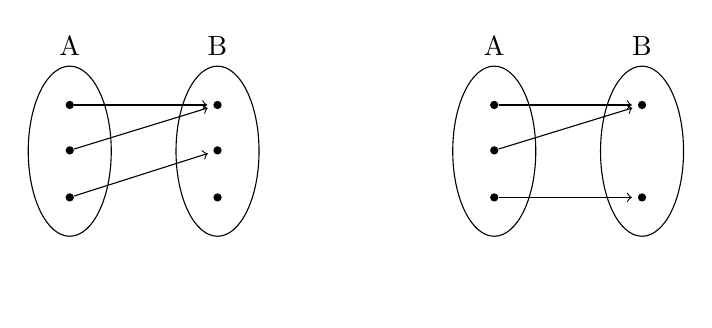
\begin{tikzpicture}
            [
            group/.style={ellipse, draw, minimum height=50pt,
                minimum width=30pt, label=above:#1},
            my dot/.style={circle, fill, minimum width=3pt, inner sep=0pt}
            ]

            \node (a0) [my dot=a] {};
            \node (b0) [below= 30pt of a0, my dot=b] {};
            \node (f0) [below=13pt of a0, my dot=c] {};
            \node (c0) [right=50pt of a0, my dot=c] {};
            \node (d0) [below= 13pt of c0, my dot=d] {};
            \node (e0) [right= 50pt of b0, my dot=e] {};

            % Replicated nodes
            \node (a1) [right=150pt of a0, my dot=a] {};
            \node (b1) [below=30pt of a1, my dot=b] {};
            \node (f1) [below=13pt of a1, my dot=c] {};
            \node (c1) [right=50pt of a1, my dot=c] {};
            \node (e1) [right=50pt of b1, my dot=e] {};

            \foreach \i in {0, 1}{
                \node [fit=(a\i) (b\i), group=A] {};
                \node [fit=(c\i) (e\i), group=B] {};
            }

            \draw [->, shorten >=2pt] (a0) -- (c0);
            \draw [->, shorten >=2pt] (f0) -- (c0);
            \draw [->, shorten >=2pt] (b0) -- (d0);

            \draw [->, shorten >=2pt] (a1) -- (c1);
            \draw [->, shorten >=2pt] (f1) -- (c1);
            \draw [->, shorten >=2pt] (b1) -- (e1);

            \node (space) [below=1cm of e1] {};

        \end{tikzpicture}
        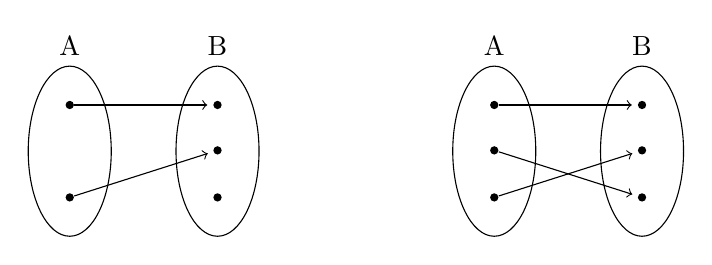
\begin{tikzpicture}
            [
            group/.style={ellipse, draw, minimum height=50pt,
                minimum width=30pt, label=above:#1},
            my dot/.style={circle, fill, minimum width=3pt, inner sep=0pt}
            ]

            \node (a0) [my dot=a] {};
            \node (b0) [below= 30pt of a0, my dot=b] {};
            \node (c0) [right=50pt of a0, my dot=c] {};
            \node (d0) [below= 13pt of c0, my dot=d] {};
            \node (e0) [right= 50pt of b0, my dot=e] {};

            % Replicated nodes
            \node (a1) [right=150pt of a0, my dot=a] {};
            \node (b1) [below=30pt of a1, my dot=b] {};
            \node (f1) [below=13pt of a1, my dot=c] {};
            \node (c1) [right=50pt of a1, my dot=c] {};
            \node (d1) [below=13pt of c1, my dot=d] {};
            \node (e1) [right=50pt of b1, my dot=e] {};

            \foreach \i in {0, 1}{
                \node [fit=(a\i) (b\i), group=A] {};
                \node [fit=(c\i) (e\i), group=B] {};
            }

            \draw [->, shorten >=2pt] (a0) -- (c0);
            \draw [->, shorten >=2pt] (b0) -- (d0);

            \draw [->, shorten >=2pt] (a1) -- (c1);
            \draw [->, shorten >=2pt] (f1) -- (e1);
            \draw [->, shorten >=2pt] (b1) -- (d1);

        \end{tikzpicture}  
        
        \caption{\label{fig:figure1} Examples of functions.}
    \end{figure}


    If a function $f: A \rightarrow A$ mapping a set to itself
    is a bijection,
    then it is also \textbf{permutation} of $A$,
    as the elements are basically being shuffled.
    All permutations are bijections. \\

    
    Furthermore, a function $f$ must have a \textbf{left inverse}
    if and only if it is injective.
    A left inverse is a function $g: B \rightarrow A$
    such that $g \circ f$ is the identity mapping $ID_A$. \\
    The reason the function must be injective is that,
    had it not been,
    $f$ would have mapped multiple elements of $A$
    to the same element of $B$,
    and that would imply that $g$ would have to map each element
    of $B$ to more than one element of $A$
    in order for $g \circ f$ to be $ID_A$,
    meaning $g$ wouldn't be well defined
    (for $g$ to be well defined,
    each element of $B$ must have exactly one mapping),
    and thus not a function. \\

    Moreover, a function $f$ must have a \textbf{right inverse}
    if and only if it is surjective.
    A right inverse is a function $g: B \rightarrow A$
    such that $f \circ g$ is the identity mapping $ID_B$. \\
    The reason the function must be surjective is that,
    had it not been,
    $f$ would not have associated all elements of $B$ with a mapping,
    and that would imply that $g$ would have
    no mappings for some elements of $B$
    in order for $f \circ g$ to be $ID_B$,
    meaning $g$ wouldn't be well defined
    (for $g$ to be well defined,
    each element of $B$ must have exactly one mapping),
    meaning $g$ wouldn't be well defined,
    and thus not a function. \\

    Finally, a function $f$ must have a \textbf{two-sided inverse}
    if and only if it is bijective.
    A right inverse is a function $g: B \rightarrow A$
    such that $f \circ g = ID_B$ and $g \circ f = ID_A$.
    The reason the function must be bijective 
    is that, had it not been,
    the conditions $f \circ g = ID_B$ and $g \circ f = ID_A$
    would each have implied that
    $g$ has no mappings, or multiple mappings,
    of elements of $B$, respectively. \\
    A two-sided inverse of $f$ is denoted by $f^{-1}$. \\
    If we have bijective mapping $f: A \rightarrow A$ from a set to itself,
    then $f^{-1} \circ f = f \circ f^{-1} = ID_A$. \\

    When $A \subseteq B$,
    and there exists a function $f: B \to C$,
    then there must exist a function $g: A \to C$,
    which maps all elements of $A$ as it would those in $B$
    (as they all belong to $B$) as well.
    This is called a \textbf{restriction} of $f$ to $A$.
    We denote it using $f|_A$. \\
    Note that $f|_A$ is unique,
    as there is only one way it can map elements of $A$;
    the same way it maps the elements of $B$ also in $A$. \\

    Likewise, if we have $A \subseteq B$,
    and there exists a function $g: A \to C$,
    then there is a possibility that there exists a function
    $f: B \to C$ that maps all elements in $B$ that are also 
    in $A$ in the same way that $f$ does.
    In other words, such that $g(a) = f|_A(a)$ for all $a \in A$. \\
    This is called an \textbf{extension} of $f$ to $B$,
    and unlike restrictions, it doesn't automatically exist,
    and may not exist at all.
    It also doesn't have to be unique,
    if $f$ maps the elements of $B$ also in $A$ in the same
    way $g$ does,
    it can still map all other elements of $B$ ($B - A$)
    however it wants to, 
    meaning several functions $f$ may exists such that 
    $g = f|_A$. \\


    \subsection*{Equivalence and Partitions}
    We already defined a binary relation between two non-empty sets
    $A$ and $B$. \\
    A relation between the set $A$ and itself 
    (a subset of $A \times A$)
    is said to be an \textbf{equivalence relation} if 
    \begin{itemize}[label=$\diamond$]
        \item 
            It is \textbf{reflexive},
            meaning that it contains $(a, a)$ $\forall a \in A$.
            In other words, it means all elements are
            associated with themseleves; $a \sim a$.
        \item 
            It is \textbf{symmetric},
            meaning that if the relation contains $(a, b)$,
            it must also contain $(b, a)$. 
            In other words, it means that if $a$ is associated
            with $b$, then $b$ is associated with $a$;
            $a \sim b$ implies $b \sim a$.
        \item
            It is \textbf{transitive},
            meaning that if the relation contains $(a, b)$
            and $(b, c)$,
            then it must also contain $(a, c)$.
            In other words, it means that if $a$ is associated
            with $b$, and $b$ is associated with $c$,
            then $a$ is associated with $c$.
            So $a \sim b$ and $b \sim c$ implies $a \sim c$.
    \end{itemize} 
    So an equivalence relation is not any association of elements,
    but an association of elements that we consider to be the same.
    The three rules we just saw ensure this sameness.
    Reflexivity ensures an element is the same as itself,
    which it obviously is.
    Symmetry ensures that no elements can be both the same
    and not the same as another based on the order of operands.
    And transitivity ensures that if an element is the same to as second,
    and that element is the same as a third,
    that the first element is the same as the third by extension. \\
    Note that not all elements need have any equivalents
    aside from themselves. \\
    A good example is the $=$ operator in a set
    such as the integers $\Z$. \\
    
    If $\sim$ defines an equivalence relation on $A$,
    then \textbf{equivalence class} of $a \in A$
    is the set of elements that are equivalent to $A$
    (the set of elements which are associated with $a$ by the relation). \\
    All the elements of this class are equivalent to $a$,
    and by transitivity, to each other.
    In fact, if $C$ is the equivalence class of $a$,
    and $x \in C$, then the equivalence class of $x$ is also $C$,
    which we can prove: \\
    Suppose $C$ is the equivalence class of $a$,
    and $x \in C$.
    Now let's take $D$ to be the equivalence class of $x$.
    Since $x \in A$,
    then by transitivity all elements equivalent to $a$
    are equivalent to $x$,
    so all elements of $C$ are in $D$,
    so $C \subseteq D$.
    Moreover, by symmetry, since $x$ is equivalent to $a$,
    $a$ is also equivalent to $x$,
    so by transitivity all elements of $D$ are equivalent to $a$,
    so all elements of $D$ are part of $C$,
    so $D \subseteq C$.
    Since $C \subseteq D$ and $D \subseteq C$,
    it must be that $C = D$,
    completing the proof. \\
    This means that any member of an equivalence class
    can represent the whole class
    (can be used to find the class, or act as a representative of it)
    as the equivalence class of all of the members is the class itself.
    Thus we say that all elements in an equivalence class
    are \textbf{representatives} of the class. \\

    A \textbf{partition} of a set $A$ is a collection
    of non-empty subsets $\{ A_i \mid i \in I \}$
    (where $I$ is some indexing set) such that:
    \begin{itemize}[label=$\diamond$]
        \item 
            $A = \bigcup_{i \in I} A_i$.
        \item 
            $A_i \cap A_j = \emptyset \text{ if } i \neq j$.
    \end{itemize}
    In other words,
    it's a way of dividing the set $A$ into disjoint subsets
    without leaving out any elements. \\

    Partitions and equivalence classes represent the same thing. \\
    On one hand, any partition can be turned into 
    an equivalence class by making all elements of disjoint subsets $A_i$
    equivalent.
    All the properties of equivalence
    would automatically be satisfied. \\
    On the other hand,
    any equivalence relation partitions a set.
    Since $a \sim a$ for all $a \in A$,
    this ensures that all elements of $A$ are in some class,
    which means that the union of equivalence classes is $A$.
    Moreover, if $a \sim b$,
    then they must be in the same equivalence class.
    If $a$ is in two equivalence classes $C$ and $D$,
    then they must be the same equivalence class
    by transitivity;
    which means all equivalence classes have to be disjoint. \\


\end{document}
